% Provenance (never printed): see sources/outline_sources.md (Year 1: internal
% structure of the Earth from seismology; reference model; density, gravity and
% pressure inside the Earth; mantle mineralogy; lithosphere and asthenosphere).
% Curves from figdata/bachelor-1/prem_profiles.py (shared dataset data:prem) and
% figdata/bachelor-1/refraction.py (generic two-layer crust); exercise and problem
% values in the Book 3 scratch calculator calc/ch09.py.
\chapter{स्तरित पृथ्वी}\label{ch:b1:layered-earth}

8 अक्तूबर 1909 को ज़ाग्रेब के दक्षिण-पूर्व में स्थित कुपा घाटी में एक भूकंप आया।
% ledger: skoko:mohorovicic
वहाँ की वेधशाला चलाने वाले आंद्रिया मोहोरोविचिच ने यूरोप भर में दर्ज भूकंपलेख इकट्ठे किए और एक अजीब बात देखी: उपरिकेंद्र से कुछ सौ किलोमीटर तक पहला कंपन एक तरह से आया, पर उससे दूर दूसरे प्रकार का पहला आगमन हावी हो गया, मानो ऊर्जा का एक हिस्सा गहराई में किसी तेज़ मार्ग पर जा निकला हो। उन्होंने इसे लगभग पचास किलोमीटर नीचे की एक सीमा से समझाया, जिसके नीचे तरंगें तेज़ चलती हैं: \omterm{def:b1:layered-earth:layers}{भूपर्पटी} का आधार। एक सदी के ऐसे अभिलेख, जिनकी संख्या लाखों में है, उस पहली सीमा को पूरी पृथ्वी के एक संदर्भ मॉडल में बदल चुके हैं, परत-दर-परत, उसके वेगों, घनत्व, गुरुत्व और केंद्र तक के दाब के साथ। यह अध्याय दिखाता है कि यात्रा-समयों से कोई सीमा कैसे खोजी जाती है, संदर्भ मॉडल क्या कहता है, केवल भूकंपीय वेगों से घनत्व-परिच्छेदिका कैसे खींची जाती है और पृथ्वी के द्रव्यमान तथा जड़त्व-आघूर्ण से उसकी जाँच कैसे होती है, गहराई पर कौन-से \omterm{def:b1:rock-forming-minerals:mineral}{खनिज} \omterm{def:b1:layered-earth:layers}{प्रावार} बनाते हैं, कोर किससे बना है, और ग्रह का कठोर बाहरी आवरण कहाँ समाप्त होता है।

\begin{recall}
P तरंग एक संपीडन तरंग है, S तरंग एक कर्तन तरंग; S तरंगें द्रवों से होकर नहीं जातीं, और कोर की P और S छाया-क्षेत्र द्रव \omterm{def:b1:layered-earth:layers}{बाह्य कोर} की त्रिज्या बताते हैं (पुस्तक 2, कक्षा 11)। तरंगें किसी सीमा पर स्नेल के नियम $\sin i_1/v_1 = \sin i_2/v_2$ के अनुसार अपवर्तित होती हैं (भौतिकी)। स्थिर द्रव में दाब गहराई के साथ $\mathrm dP = \rho g\,\mathrm dz$ के अनुसार बढ़ता है (भौतिकी, विश्वविद्यालय वर्ष 1)। \omterm{def:b1:layered-earth:layers}{भूपर्पटी}, \omterm{def:b1:layered-earth:layers}{प्रावार} और कोर पुस्तक 1 (कक्षा 6) में परिचित कराए गए थे।
\end{recall}

\section{स्तरित पृथ्वी में भूकंपीय तरंगें}

भूकंपीय तरंगों की चाल चट्टान के प्रत्यास्थ मापांकों और उसके घनत्व पर निर्भर करती है। भौतिकी की पुस्तकें इन्हें सतत-प्रत्यास्थता के समीकरणों से निकालती हैं; यहाँ इन्हें ज्ञात माना गया है।

\begin{proposition}[भूकंपीय चालें]\label{prop:b1:layered-earth:speeds}
घनत्व $\rho$, आयतन-मापांक $K$ और अपरूपण-मापांक $\mu$ वाले एक समदैशिक प्रत्यास्थ ठोस में P और S तरंगें इन चालों से चलती हैं:
\[
  v_P = \sqrt{\frac{K + \tfrac43\mu}{\rho}}, \qquad v_S = \sqrt{\frac{\mu}{\rho}}.
\]
द्रव में $\mu = 0$ होता है: $v_S = 0$ और कोई S तरंग संचरित नहीं होती।
\end{proposition}
\admitted

चूँकि $K$ और $\mu$ धनात्मक हैं, $v_P > v_S$ सदा होता है: PREM की \omterm{def:b1:layered-earth:layers}{भूपर्पटी} और \omterm{def:b1:layered-earth:layers}{प्रावार} में $v_P$ लगभग $1.8$ से $1.9$ गुना $v_S$ है, और P तरंगें पहले पहुँचती हैं। दोनों चालें सामान्यतः गहराई के साथ बढ़ती हैं, क्योंकि दाब चट्टान को उसके संपीड़न की तुलना में अधिक कठोर बनाता है, जिससे किरणें सतह की ओर मुड़ती हैं; और कुछ गहराइयों पर वे अचानक उछलती हैं।

\begin{definition}[भूकंपीय असांतत्य, मोहो, कोर–प्रावार और आंतरिक-कोर सीमाएँ]
\label{def:b1:layered-earth:discontinuity}
एक \emph{भूकंपीय असांतत्य}\index{भूकंपीय असांतत्य} पृथ्वी के भीतर की वह सतह है जिस पर भूकंपीय वेग, घनत्व या दोनों एकाएक बदलते हैं, और जिसकी मोटाई भूकंपीय तरंगदैर्घ्य की तुलना में छोटी होती है। \emph{मोहोरोविचिच असांतत्य}\index{मोहोरोविचिच असांतत्य} (या \emph{मोहो}\index{मोहो}) \omterm{def:b1:layered-earth:layers}{भूपर्पटी} का आधार है, जहाँ $v_P$ लगभग \qty{8}{km.s^{-1}} तक उछलता है। \emph{कोर–प्रावार सीमा}\index{कोर–प्रावार सीमा} ठोस सिलिकेट \omterm{def:b1:layered-earth:layers}{प्रावार} और द्रव \omterm{def:b1:layered-earth:layers}{बाह्य कोर} के बीच की सतह है; \emph{आंतरिक-कोर सीमा}\index{आंतरिक-कोर सीमा} द्रव \omterm{def:b1:layered-earth:layers}{बाह्य कोर} और ठोस \omterm{def:b1:layered-earth:layers}{आंतरिक कोर} के बीच की सतह है।
\end{definition}

\subsection{परत-सीमा पर अपवर्तन}

एक परत लीजिए जिसकी मोटाई $h$ और चाल $v_1$ है, यानी \omterm{def:b1:layered-earth:layers}{भूपर्पटी}, जो चाल $v_2 > v_1$ वाले अर्ध-अंतरिक्ष, यानी \omterm{def:b1:layered-earth:layers}{प्रावार}, पर टिकी है, और सतह पर एक स्रोत। एक ग्राही पर दूरी $x$ पर तीन तरंगें पहुँचती हैं। प्रत्यक्ष तरंग परत में $v_1$ पर चलती है। परावर्तित तरंग सीमा से लौटती है। और एक किरण जो सीमा से क्रांतिक कोण $i_c$ पर टकराती है, जहाँ $\sin i_c = v_1/v_2$ है, सीमा के साथ-साथ अपवर्तित होकर चलती है, उसके ठीक नीचे के तेज़ माध्यम में चाल $v_2$ से चलती है, और अपने पूरे मार्ग में उसी कोण $i_c$ पर परत में ऊर्जा वापस भेजती है।

\begin{definition}[हेड तरंग, क्रॉसओवर दूरी]
\label{def:b1:layered-earth:head-wave}
एक \emph{हेड तरंग}\index{हेड तरंग} वह तरंग है जो किसी सीमा के साथ-साथ उसके नीचे के तेज़ माध्यम की चाल से चलती है और क्रांतिक कोण पर ऊपर की ओर निकलती है। \emph{क्रॉसओवर दूरी}\index{क्रॉसओवर दूरी} वह स्रोत-दूरी है जिससे आगे हेड तरंग प्रत्यक्ष तरंग से पहले पहुँचती है।
\end{definition}

\begin{theorem}[दो-परत पृथ्वी पर यात्रा-समय]\label{thm:b1:layered-earth:two-layer}
मोटाई $h$ और चाल $v_1$ की एक परत, जो चाल $v_2 > v_1$ वाले अर्ध-अंतरिक्ष पर टिकी है, पर, दूरी $x$ पर स्थित एक सतही स्रोत और एक सतही ग्राही के लिए निम्नलिखित प्राप्त होता है:
\[
  t_{\text{प्रत्यक्ष}} = \frac{x}{v_1}, \qquad
  t_{\text{हेड}} = \frac{x}{v_2} + \frac{2h\cos i_c}{v_1}
  \quad (x \ge 2h\tan i_c), \qquad \sin i_c = \frac{v_1}{v_2},
\]
और \omterm{def:b1:layered-earth:head-wave}{हेड तरंग} उस \omterm{def:b1:layered-earth:head-wave}{क्रॉसओवर दूरी} से आगे पहले पहुँचती है:
\[
  x_c = 2h\sqrt{\frac{v_2 + v_1}{v_2 - v_1}}.
\]
\end{theorem}

\begin{proof}
\omterm{def:b1:layered-earth:head-wave}{हेड तरंग} परत से होकर कोण $i_c$ पर नीचे जाती है, $h/\cos i_c$ लंबाई का पथ तय करती है, सीमा के साथ दूरी $x - 2h\tan i_c$ पर दौड़ती है, और $h/\cos i_c$ लंबाई के पथ से ऊपर आती है। इसका यात्रा-समय है:
\[
  t_{\text{हेड}} = \frac{2h}{v_1\cos i_c} + \frac{x - 2h\tan i_c}{v_2}
  = \frac{x}{v_2} + \frac{2h}{v_1\cos i_c}\Bigl(1 - \frac{v_1\sin i_c}{v_2}\Bigr)
  = \frac{x}{v_2} + \frac{2h}{v_1\cos i_c}\,(1 - \sin^2 i_c),
\]
अर्थात् $x/v_2 + 2h\cos i_c/v_1$। पथ तभी विद्यमान है जब क्षैतिज दूरी धनात्मक हो, $x \ge 2h\tan i_c$। दोनों समय बराबर होते हैं जब $x(1/v_1 - 1/v_2) = 2h\cos i_c/v_1$ हो; और $\cos i_c = \sqrt{v_2^2 - v_1^2}/v_2$ के साथ,
\[
  x\,\frac{v_2 - v_1}{v_1 v_2} = \frac{2h\sqrt{(v_2 - v_1)(v_2 + v_1)}}{v_1 v_2},
\]
जिससे $x_c$ मिलता है। उसके आगे हेड-तरंग रेखा, जिसकी ढलान $1/v_2$ छोटी है, प्रत्यक्ष-तरंग रेखा के नीचे रहती है।
\end{proof}

यात्रा-समय बनाम दूरी के ग्राफ़ पर प्रत्यक्ष और हेड तरंगें दो सीधी रेखाएँ हैं। उनकी ढलानें चालों के व्युत्क्रम, $1/v_1$ और $1/v_2$, हैं; हेड-तरंग रेखा को $x = 0$ तक पीछे बढ़ाने पर वह समय-अक्ष को \emph{अंतःखंड-समय} $t_i = 2h\cos i_c/v_1$ पर काटती है। परावर्तित तरंग, $t = \sqrt{x^2 + 4h^2}/v_1$, एक अतिपरवलय है जो क्रांतिक दूरी $2h\tan i_c$ पर हेड-तरंग रेखा को स्पर्श करती है, जहाँ \omterm{def:b1:layered-earth:head-wave}{हेड तरंग} जन्म लेती है (\cref{exo:b1:layered-earth:10})।

\begin{omfigure}
\begin{tabular}{@{}c@{}}
\begin{tikzpicture}
\begin{axis}[width=0.86\linewidth, axis equal image, xmin=0, xmax=260, ymin=-62, ymax=8,
  axis x line=top, axis y line=left, axis line style={-}, clip=false,
  ylabel={गहराई (km)}, ytick={-60,-35,0},
  yticklabels={60,35,0}, tick label style={font=\scriptsize}, label style={font=\small}]
\fill[brown!12] (axis cs:0,0) rectangle (axis cs:260,-35);
\fill[orange!18] (axis cs:0,-35) rectangle (axis cs:260,-62);
\draw[black!60] (axis cs:0,-35) -- (axis cs:260,-35);
\addplot[very thick, blue!70!black] table[x=x, y=z, unbounded coords=jump,
  restrict expr to domain={\coordindex}{0:1}] {figdata/out/bachelor-1-refraction-rays.dat};
\addplot[thick, dashed, green!45!black] table[x=x, y=z, unbounded coords=jump,
  restrict expr to domain={\coordindex}{3:5}] {figdata/out/bachelor-1-refraction-rays.dat};
\addplot[very thick, red!75!black] table[x=x, y=z, unbounded coords=jump,
  restrict expr to domain={\coordindex}{7:10}] {figdata/out/bachelor-1-refraction-rays.dat};
\node[font=\scriptsize, anchor=north west] at (axis cs:2,-36) {प्रावार, $v_2 = \qty{8.0}{km.s^{-1}}$};
\node[font=\scriptsize, anchor=center] at (axis cs:125,-17) {भूपर्पटी, $v_1 = \qty{6.0}{km.s^{-1}}$, $h = \qty{35}{km}$};
\node[font=\scriptsize, red!75!black, anchor=north] at (axis cs:150,-36) {मोहो के साथ चलती हेड तरंग};
\node[font=\scriptsize, green!45!black, anchor=south] at (axis cs:40,-20) {परावर्तित};
\node[font=\scriptsize, blue!70!black, anchor=north] at (axis cs:125,-1) {प्रत्यक्ष};
\fill (axis cs:0,0) circle (2pt);
\end{axis}
\end{tikzpicture}\\[2pt]
{\small (क) किरण-पथ (दूरी km में)}\\[6pt]
\begin{tikzpicture}
\begin{axis}[omrecord, width=0.86\linewidth, height=6.0cm, xmin=0, xmax=400, ymin=0, ymax=70,
  xlabel={दूरी $x$ (km)}, ylabel={यात्रा-समय $t$ (s)}, tick label style={font=\scriptsize},
  label style={font=\small}, clip=false,
  legend style={font=\scriptsize, at={(0.03,0.97)}, anchor=north west, draw=none, fill=white, fill opacity=0.85}]
\addplot[very thick, blue!70!black] table[x=x, y=t_direct] {figdata/out/bachelor-1-refraction-times.dat};
\addlegendentry{प्रत्यक्ष, ढलान $1/v_1$}
\addplot[thick, dashed, green!45!black] table[x=x, y=t_reflected] {figdata/out/bachelor-1-refraction-times.dat};
\addlegendentry{परावर्तित}
\addplot[very thick, red!75!black, unbounded coords=jump] table[x=x, y=t_head] {figdata/out/bachelor-1-refraction-times.dat};
\addlegendentry{हेड तरंग, ढलान $1/v_2$}
\addplot[thin, dotted, red!75!black, domain=0:79.37] {x/8 + 7.717};
\draw[black!60, densely dashed] (axis cs:185.2,0) -- (axis cs:185.2,30.87);
\node[font=\scriptsize, anchor=north west] at (axis cs:187,8) {$x_c = \qty{185}{km}$};
\node[font=\scriptsize, anchor=east, red!75!black] at (axis cs:-3,7.7) {$t_i$};
\end{axis}
\end{tikzpicture}\\[2pt]
{\small (ख) यात्रा-समय}
\end{tabular}

\par\smallskip{\small \qty{35}{km} मोटी \omterm{def:b1:layered-earth:layers}{भूपर्पटी} में, \qty{6.0}{km.s^{-1}} चाल से, \qty{8.0}{km.s^{-1}} वाले \omterm{def:b1:layered-earth:layers}{प्रावार} पर अपवर्तन ((क) वास्तविक पैमाने पर)। (क) प्रत्यक्ष तरंग सतह के साथ चलती है; परावर्तित तरंग जो दिखाई गई है वह क्रांतिक कोण \ang{48.6} पर \omterm{def:b1:layered-earth:discontinuity}{मोहो} से टकराने वाली तरंग है; \omterm{def:b1:layered-earth:head-wave}{हेड तरंग} \omterm{def:b1:layered-earth:discontinuity}{मोहो} के साथ चलती है और उसी कोण पर लौटती है। (ख) आगमन-समय: \omterm{def:b1:layered-earth:head-wave}{हेड तरंग} क्रांतिक दूरी \qty{79}{km} पर प्रकट होती है, परावर्तन को स्पर्श करती हुई, और \omterm{def:b1:layered-earth:head-wave}{क्रॉसओवर दूरी} \qty{185}{km} पर प्रत्यक्ष तरंग को पीछे छोड़ देती है। बिंदुकित विस्तार अंतःखंड-समय $t_i = \qty{7.7}{s}$ देता है।}
\end{omfigure}

\begin{method}[अपवर्तन-परिच्छेदिका से सीमा की गहराई]\label{met:b1:layered-earth:moho}
\begin{enumerate}
  \item प्रथम-आगमन समयों को दूरी के विरुद्ध ग्राफ़ पर खींचिए, और स्रोत के निकट के आगमनों से होकर एक सीधी रेखा तथा दूर के आगमनों से होकर दूसरी रेखा खींचिए।
  \item व्युत्क्रम ढलानें $v_1$ और $v_2$ देती हैं; फिर $\sin i_c = v_1/v_2$।
  \item दूर की रेखा का अंतःखंड-समय $t_i$ पढ़िए, जो $x = 0$ पर है, और $h = t_i v_1/(2\cos i_c)$ परिकलित कीजिए; उसे \omterm{def:b1:layered-earth:head-wave}{क्रॉसओवर दूरी} से जाँचिए, $h = \tfrac12 x_c\sqrt{(v_2 - v_1)/(v_2 + v_1)}$।
  \item सीमा केवल तभी मिलती है जब $v_2 > v_1$ हो: एक धीमी परत जो तेज़ परत के नीचे हो, कोई \omterm{def:b1:layered-earth:head-wave}{हेड तरंग} नहीं बनाती और छिपी रहती है।
\end{enumerate}
\end{method}

मोहोरोविचिच के आगमन के दो प्रकार ठीक इन्हीं दो रेखाओं के थे: स्रोत के निकट \omterm{def:b1:layered-earth:layers}{भूपर्पटी} में प्रत्यक्ष तरंग, और दूर \omterm{def:b1:layered-earth:layers}{प्रावार} के ऊपरी भाग के साथ \omterm{def:b1:layered-earth:head-wave}{हेड तरंग}। उस क्षेत्र में \omterm{def:b1:layered-earth:layers}{भूपर्पटी} की मोटाई के बारे में उनका आंकड़ा, \qty{54}{km}, अपने परिमाण-क्रम में पुष्ट हुआ है, किंतु \omterm{def:b1:layered-earth:discontinuity}{मोहो} की गहराई स्थान-स्थान पर बदलती है। महासागरों के नीचे \omterm{def:b1:layered-earth:layers}{भूपर्पटी} केवल लगभग \qty{5}{km} मोटी है; महाद्वीपों के नीचे उसका औसत लगभग \qty{30}{km} है, और बड़ी पर्वत-शृंखलाओं के नीचे वह कहीं अधिक मोटी है। अपने संदर्भ मॉडल के लिए PREM ने \omterm{def:b1:layered-earth:discontinuity}{मोहो} को महासागरों के नीचे समुद्र-तल से \qty{11}{km} नीचे और महाद्वीपों के नीचे \qty{35}{km} पर लिया।
% ledger: skoko:mohorovicic, usgs:crust-thickness, prem:moho-average

\begin{history}[आंद्रिया मोहोरोविचिच]
\begin{minipage}[t]{0.76\linewidth}\vspace{0pt}
% ledger: skoko:mohorovicic
आंद्रिया मोहोरोविचिच (1857--1936) मौसम-विज्ञान से भूकंप-विज्ञान में आए: पहले शिक्षक, फिर 1891 से 1921 तक ज़ाग्रेब की मौसम-वेधशाला के निदेशक; उन्होंने अपना अंतिम मौसम-विज्ञान अध्ययन 1901 में प्रकाशित किया। 8 अक्तूबर 1909 के कुपा घाटी भूकंप के भूकंपलेखों पर उन्हें P और S चरणों के दो अलग-अलग जोड़े मिले: स्रोत के निकट एक प्रकार का पहला कंपन पहले पहुँचा, और दूर दूसरा, जो गहराई में तेज़ चला था। इन दो आगमनों को एक प्रत्यक्ष तरंग और एक सीमा के नीचे से अपवर्तित तरंग पढ़ने से उन्हें वह सीमा मिली जो आज उनके नाम से जानी जाती है, और \omterm{def:b1:layered-earth:layers}{भूपर्पटी} की मोटाई का पहला माप भी।
\end{minipage}\hfill
\begin{minipage}[t]{0.2\linewidth}\vspace{0pt}
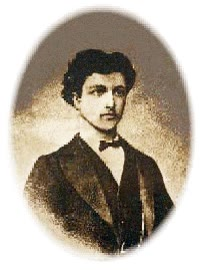
\includegraphics[width=\linewidth]{images/book3/b1-mohorovicic.jpg}

{\scriptsize आंद्रिया मोहोरोविचिच। सार्वजनिक क्षेत्र।}
\end{minipage}
\end{history}

\section{एक संदर्भ पृथ्वी मॉडल}

इसी तर्क को, जो लाखों यात्रा-समयों और पृथ्वी के मुक्त दोलनों के कालों पर लागू होता है (पूरा ग्रह किसी बड़े भूकंप के बाद घंटी की तरह गूँजता है), हर गहराई पर चालें मिलती हैं।

\begin{definition}[संदर्भ पृथ्वी मॉडल]\label{def:b1:layered-earth:reference-model}
एक \emph{संदर्भ पृथ्वी मॉडल}\index{संदर्भ पृथ्वी मॉडल} एक गोलीय-सममित पृथ्वी है, जिसे भूकंपीय चालों $v_P(r)$, $v_S(r)$, घनत्व $\rho(r)$ और, सबसे पूर्ण मॉडलों में, क्षीणन के रूप में दिया जाता है; ये सब केवल त्रिज्या $r$ के फलन हैं। यह मॉडल प्रेक्षित यात्रा-समयों, मुक्त-दोलन कालों, पृथ्वी के द्रव्यमान और उसके जड़त्व-आघूर्ण से मेल खाता है। सबसे व्यापक रूप से प्रयुक्त मॉडल PREM है, यानी प्रारंभिक संदर्भ पृथ्वी मॉडल (1981)।
\end{definition}

PREM को पृथ्वी की त्रिज्या \qty{6371}{km}, द्रव्यमान \qty{5.974e24}{kg} और जड़त्व-आघूर्ण-गुणांक $0.3308$ पर फ़िट किया गया था। वह ग्रह को कुछ क्षेत्रों में बाँटता है जिन्हें असांतत्य जोड़ते हैं, और उसकी परिच्छेदिकाएँ (नीचे का चित्र) मुख्य परतों को एक नज़र में दिखाती हैं।

\begin{definition}[भूपर्पटी, प्रावार, बाह्य कोर, आंतरिक कोर]\label{def:b1:layered-earth:layers}
\emph{भूपर्पटी}\index{भूपर्पटी} \omterm{def:b1:layered-earth:discontinuity}{मोहो} के ऊपर की बाहरी सिलिकेट परत है। \emph{प्रावार}\index{प्रावार} \omterm{def:b1:layered-earth:discontinuity}{मोहो} और \omterm{def:b1:layered-earth:discontinuity}{कोर–प्रावार सीमा} के बीच का ठोस सिलिकेट कवच है, जो लगभग \qty{2891}{km} गहराई पर है। \emph{बाह्य कोर}\index{बाह्य कोर} \omterm{def:b1:layered-earth:discontinuity}{कोर–प्रावार सीमा} और \omterm{def:b1:layered-earth:discontinuity}{आंतरिक-कोर सीमा} के बीच का द्रव धात्विक कवच है, जो लगभग \qty{5150}{km} गहराई पर है। \emph{आंतरिक कोर}\index{आंतरिक कोर} उसके नीचे का ठोस धात्विक गोला है, जिसकी त्रिज्या लगभग \qty{1220}{km} है।
\end{definition}

\begin{omfigure}
\begin{tikzpicture}
\begin{axis}[omrecord, omdepth, width=0.62\linewidth, height=5.4cm, xmin=0, xmax=14, ymin=0, ymax=6371,
  xlabel={वेग (\unit{km.s^{-1}}) या घनत्व (\unit{g.cm^{-3}})}, ylabel={गहराई (km)},
  ytick={0,1000,...,6000}, tick label style={font=\scriptsize}, label style={font=\small},
  clip=false, legend style={font=\scriptsize, at={(0.02,0.80)}, anchor=north west, draw=none, fill=white}]
\addplot[very thick, blue!70!black] table[x=vp, y=depth] {figdata/out/bachelor-1-prem_profiles-profiles.dat};
\addlegendentry{$v_P$}
\addplot[very thick, red!75!black] table[x=vs, y=depth] {figdata/out/bachelor-1-prem_profiles-profiles.dat};
\addlegendentry{$v_S$}
\addplot[very thick, black!70, densely dashed] table[x=rho, y=depth] {figdata/out/bachelor-1-prem_profiles-profiles.dat};
\addlegendentry{$\rho$}
\draw[black!35] (axis cs:0,670) -- (axis cs:14,670) node[right, font=\scriptsize, black] {670 km};
\draw[black!35] (axis cs:0,2891) -- (axis cs:14,2891) node[right, font=\scriptsize, black] {कोर–प्रावार सीमा};
\draw[black!35] (axis cs:0,5149.5) -- (axis cs:14,5149.5) node[right, font=\scriptsize, black] {आंतरिक-कोर सीमा};
\node[font=\scriptsize, anchor=west] at (axis cs:14,1700) {प्रावार};
\node[font=\scriptsize, anchor=west] at (axis cs:14,4000) {बाह्य कोर (द्रव)};
\node[font=\scriptsize, anchor=west] at (axis cs:14,5800) {आंतरिक कोर (ठोस)};
\end{axis}
\end{tikzpicture}

\par\smallskip{\small PREM: P और S तरंगों की चालें और घनत्व गहराई के विरुद्ध। S चाल द्रव \omterm{def:b1:layered-earth:layers}{बाह्य कोर} में शून्य तक गिरती है और ठोस \omterm{def:b1:layered-earth:layers}{आंतरिक कोर} में छोटी होकर फिर प्रकट होती है; \omterm{def:b1:layered-earth:discontinuity}{कोर–प्रावार सीमा} पर घनत्व लगभग दोगुना हो जाता है, जबकि $v_P$ 13.7 से गिरकर \qty{8.1}{km.s^{-1}} हो जाता है; \qty{400}{km} और \qty{670}{km} के पास की छलांगें संक्रमण-क्षेत्र की सीमा बनाती हैं।}
\end{omfigure}

\begin{table}[htbp]
\centering
\footnotesize
\setlength{\tabcolsep}{3pt}
\begin{tabular}{>{\raggedright\arraybackslash}p{0.2\linewidth}rr>{\raggedright\arraybackslash}p{0.47\linewidth}}
\hline
PREM में सीमा & गहराई (km) & त्रिज्या (km) & क्या बदलता है \\
\hline
\omterm{def:b1:layered-earth:discontinuity}{मोहो} & 24.4 & 6346.6 & ऊपर \omterm{def:b1:layered-earth:layers}{भूपर्पटी}, नीचे पेरिडोटाइट; $v_P$ 6.8 से 8.1 \\
220-km असांतत्य & 220 & 6151 & PREM में \omterm{def:b1:layered-earth:lithosphere}{निम्न-वेग क्षेत्र} का आधार \\
400-km असांतत्य & 400 & 5971 & \omterm{def:b1:rock-forming-minerals:groups}{ओलिवीन} से वैडस्लेयाइट (अधिकांश अध्ययनों में \qty{410}{km}) \\
670-km असांतत्य & 670 & 5701 & रिंगवुडाइट से ब्रिजमैनाइट और फ़ेरोपेरिक्लेज़ (अधिकांश अध्ययनों में \qty{660}{km}) \\
\omterm{def:b1:layered-earth:discontinuity}{कोर–प्रावार सीमा} & 2891 & 3480 & सिलिकेट से द्रव लोहा; $v_S$ 7.3 से 0; $\rho$ 5.57 से 9.90 \\
\omterm{def:b1:layered-earth:discontinuity}{आंतरिक-कोर सीमा} & 5149.5 & 1221.5 & द्रव से ठोस लोहा; $v_S$ 0 से 3.5; $\rho$ 12.17 से 12.76 \\
\hline
\end{tabular}
\caption{PREM के मुख्य असांतत्य (चालें \unit{km.s^{-1}} में, घनत्व \unit{g.cm^{-3}} में)। PREM \omterm{def:b1:layered-earth:layers}{भूपर्पटी} को \qty{24.4}{km} पर औसत करता है; वास्तविक भूपर्पटियाँ महासागरों के नीचे लगभग \qty{5}{km} से लेकर पर्वत-शृंखलाओं के नीचे कई दर्जन किलोमीटर तक होती हैं।}
% ledger: usgs:crust-thickness
\label{tab:b1:layered-earth:prem}
\end{table}

इस परिच्छेदिका में दो तथ्य सीधे प्रेक्षित होते हैं। \omterm{def:b1:layered-earth:layers}{बाह्य कोर} में $v_S$ का लुप्त होना ऊपर याद किया गया S-छाया-क्षेत्र है: S तरंगें कोर में केवल P तरंगों के रूप में प्रवेश करती हैं, कोर कर्तन नहीं संचरित कर सकता, इसलिए वह द्रव है। और \omterm{def:b1:layered-earth:layers}{आंतरिक कोर} S तरंगें संचरित करता है, धीरे-धीरे: वह ठोस है। यह दूसरा तथ्य उन दुर्बल P आगमनों से आया जहाँ कोई P तरंग नहीं होनी चाहिए थी।

\begin{history}[इंगे लेमन और आंतरिक कोर]
% ledger: hjortenberg:lehmann
\begin{minipage}[t]{0.76\linewidth}\vspace{0pt}
इंगे लेमन (1888--1993), डेनिश भूमापन संस्थान के भूकंप-विज्ञान विभाग की प्रमुख, 1929 के न्यूज़ीलैंड के बुलर भूकंप के अभिलेखों का अध्ययन कर रही थीं और उन्हें P तरंगें छाया-क्षेत्र के भीतर पहुँचती मिलीं, जहाँ कोर उन्हें दूर मोड़ देता। 1936 के एक पर्चे में, जिसका शीर्षक सबसे छोटा था, \emph{P$'$}, उन्होंने दिखाया कि यदि कोर में एक छोटा \omterm{def:b1:layered-earth:layers}{आंतरिक कोर} हो जिसमें P चाल अधिक हो, तो ये आगमन समझाए जा सकते हैं, क्योंकि वह ऊर्जा का एक भाग सतह की ओर वापस भेजता है। उनका \omterm{def:b1:layered-earth:layers}{आंतरिक कोर} अब ठोस जाना जाता है, और पृथ्वी के ठंडे होने के साथ धीरे-धीरे बढ़ता है। उन्होंने लगभग \qty{220}{km} पर वह असांतत्य भी खोजा जो उनके नाम पर है।
\end{minipage}\hfill
\begin{minipage}[t]{0.2\linewidth}\vspace{0pt}
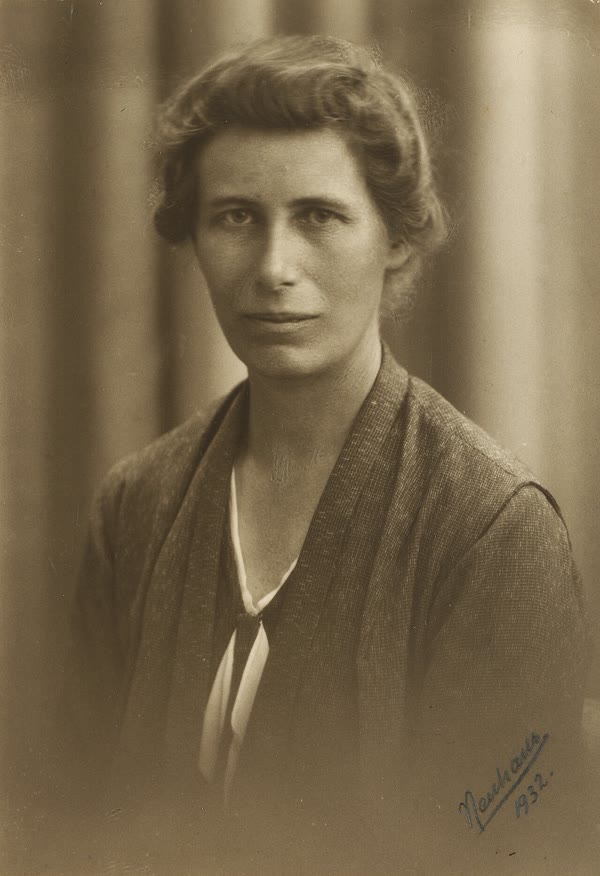
\includegraphics[width=\linewidth]{images/book3/b1-lehmann.jpg}

{\scriptsize 1932 में इंगे लेमन, Even Neuhaus द्वारा। सार्वजनिक क्षेत्र।}
\end{minipage}
\end{history}

\section{घनत्व, गुरुत्व और दाब भूकंपीय आँकड़ों से}

भूकंपीय चालें दो संयोजन देती हैं, मापांकों और घनत्व के, स्वयं घनत्व नहीं। एक तीसरा संबंध इस धारणा से आता है कि एक समान संघटन की परत के भीतर चट्टान केवल ऊपर की चट्टान के भार से संपीड़ित होती है।

\begin{definition}[भूकंपीय प्राचल]\label{def:b1:layered-earth:seismic-parameter}
किसी गहराई पर \emph{भूकंपीय प्राचल}\index{भूकंपीय प्राचल} है
\[
  \Phi = v_P^2 - \tfrac43 v_S^2 = \frac{K}{\rho},
\]
घनत्व से विभाजित आयतन-मापांक, जो केवल दो भूकंपीय चालों से परिकलित होता है (\cref{prop:b1:layered-earth:speeds})।
\end{definition}

\begin{theorem}[एडम्स–विलियम्सन समीकरण]\label{thm:b1:layered-earth:adams-williamson}
एक समान संघटन के क्षेत्र में, द्रवस्थैतिक साम्य में, रुद्धोष्म संपीड़ित होने पर, घनत्व त्रिज्या के साथ इस प्रकार बदलता है:
\[
  \frac{\mathrm d\rho}{\mathrm dr} = -\frac{\rho(r)\,g(r)}{\Phi(r)},
\]
जहाँ $g(r)$ त्रिज्या $r$ पर गुरुत्व है।
\end{theorem}

\begin{proof}
द्रवस्थैतिक साम्य $\mathrm dP/\mathrm dr = -\rho g$ देता है (स्मरण, जहाँ $\mathrm dz = -\mathrm dr$ है)। आयतन-मापांक उस संपीड़न के लिए $K = \rho\,\mathrm dP/\mathrm d\rho$ से परिभाषित होता है; एक ऐसी चट्टान के लिए जिसका संघटन स्थिर है और जो ऊष्मा के आदान-प्रदान के बिना संपीड़ित होती है, यह रुद्धोष्म मापांक है जिसे भूकंपीय तरंगें मापती हैं, अतः $\mathrm d\rho/\mathrm dP = \rho/K$। शृंखला-नियम से,
\[
  \frac{\mathrm d\rho}{\mathrm dr} = \frac{\mathrm d\rho}{\mathrm dP}\,
  \frac{\mathrm dP}{\mathrm dr} = \frac{\rho}{K}\,(-\rho g) = -\frac{\rho g}{K/\rho}
  = -\frac{\rho g}{\Phi}. \qedhere
\]
\end{proof}

यह समीकरण किसी असांतत्य पर विफल हो जाता है, जहाँ संघटन या क्रिस्टल-संरचना बदलती है, और जहाँ तापमान रुद्धोष्म रेखा से हटता है; पर असांतत्यों के बीच यह गहराई के साथ घनत्व की देखी गई वृद्धि को बहुत अच्छी तरह समझाता है (नीचे के चित्र का भाग (ग))। हर क्षेत्र के ऊपर के एक घनत्व से आरंभ करके, उसे नीचे की ओर समाकलित करके, और आरंभिक मानों को तब तक समायोजित करके कि द्रव्यमान और जड़त्व-आघूर्ण सही निकलें, पहले घनत्व-मॉडल बने। दोनों वैश्विक संख्याएँ घनत्व के समाकल हैं।

\begin{proposition}[द्रव्यमान, गुरुत्व, दाब और जड़त्व-आघूर्ण]
\label{prop:b1:layered-earth:integrals}
त्रिज्या $R$ और घनत्व $\rho(r)$ वाली एक गोलीय-सममित पृथ्वी के लिए, त्रिज्या $r$ के भीतर का द्रव्यमान, गुरुत्व, दाब और केंद्र से होकर गुज़रती अक्ष के परितः जड़त्व-आघूर्ण हैं:
\[
  m(r) = \int_0^r 4\pi s^2\rho(s)\,\mathrm ds, \quad
  g(r) = \frac{G\,m(r)}{r^2}, \quad
  P(r) = \int_r^R \rho(s)\,g(s)\,\mathrm ds, \quad
  I = \frac{8\pi}{3}\int_0^R \rho(r)\,r^4\,\mathrm dr.
\]
\end{proposition}

\begin{proof}
एक त्रिज्या $s$ और मोटाई $\mathrm ds$ वाले पतले कोश का आयतन $4\pi s^2\,\mathrm ds$ होता है, अतः पहला समाकल। किसी त्रिज्या के बाहर के गोलीय-सममित पिंड का गुरुत्व उसके भीतर के द्रव्यमान के समान होता है, जो केंद्र पर संकेंद्रित है, और $r$ के बाहर के कोश कोई शुद्ध बल नहीं लगाते (कोश-प्रमेय, जिसे भौतिकी की पुस्तकों से स्वीकार किया गया है); अतः $g(r)$। साम्य-समीकरण को सतह से समाकलित करने पर, जहाँ $P = 0$ है, $P(r)$ मिलता है। जड़त्व-आघूर्ण के लिए, द्रव्यमान $\mathrm dm$ और त्रिज्या $r$ वाला एक पतला गोलीय कोश, अक्षों $x$, $y$, $z$ के परितः ऐसे आघूर्ण रखता है जिनका योग $\int (y^2 + z^2) + (z^2 + x^2) + (x^2 + y^2)\,\mathrm dm = 2r^2\,\mathrm dm$ है; समरूपता से तीनों बराबर हैं, अतः प्रत्येक $\tfrac23 r^2\,\mathrm dm$ है। $\mathrm dm = 4\pi r^2\rho\,\mathrm dr$ के साथ कोशों को जोड़ने पर $I$ मिलता है।
\end{proof}

एकसमान घनत्व वाले गोले के लिए $I = \tfrac{8\pi}{15}\rho R^5 = 0.4\,MR^2$ है। पृथ्वी का गुणांक $I/MR^2 = 0.3308$ छोटा है: उसका द्रव्यमान केंद्र की ओर संकेंद्रित है, और यही सघन कोर का पहला तर्क है। केवल PREM के घनत्व से परिकलित समाकल \qty{5.976e24}{kg} का द्रव्यमान देते हैं (मापे गए \qty{5.972e24}{kg} से \qty{0.06}{\percent} अधिक), गुणांक $0.3309$, और \qty{364}{GPa} का केंद्रीय दाब, वह मान जो PREM के साथ \qty{0.1}{\percent} तक सारणीबद्ध है।

\begin{omfigure}
\begin{tabular}{@{}c@{\hspace{2mm}}c@{\hspace{2mm}}c@{}}
\begin{tikzpicture}
\begin{axis}[omrecord, omdepth, width=0.35\linewidth, height=7.0cm, xmin=0, xmax=12, ymin=0, ymax=6371,
  xlabel={$g$ (\unit{m.s^{-2}})}, ylabel={गहराई (km)}, ytick={0,1000,...,6000}, xtick={0,4,8,12},
  tick label style={font=\scriptsize}, label style={font=\small}]
\addplot[very thick, blue!70!black] table[x=g, y=depth] {figdata/out/bachelor-1-prem_profiles-functionals.dat};
\draw[black!35] (axis cs:0,2891) -- (axis cs:12,2891);
\draw[black!35] (axis cs:0,5149.5) -- (axis cs:12,5149.5);
\node[font=\scriptsize, anchor=south west] at (axis cs:0.3,2891) {CMB};
\node[font=\scriptsize, anchor=south west] at (axis cs:0.3,5149.5) {ICB};
\end{axis}
\end{tikzpicture}
&
\begin{tikzpicture}
\begin{axis}[omrecord, omdepth, width=0.35\linewidth, height=7.0cm, xmin=0, xmax=400, ymin=0, ymax=6371,
  xlabel={दाब $P$ (GPa)}, ytick={0,1000,...,6000}, yticklabels={}, xtick={0,200,400},
  tick label style={font=\scriptsize}, label style={font=\small}]
\addplot[very thick, red!75!black] table[x=P, y=depth] {figdata/out/bachelor-1-prem_profiles-functionals.dat};
\draw[black!35] (axis cs:0,2891) -- (axis cs:400,2891);
\draw[black!35] (axis cs:0,5149.5) -- (axis cs:400,5149.5);
\node[font=\scriptsize, anchor=south west] at (axis cs:150,2891) {\qty{136}{GPa}};
\node[font=\scriptsize, anchor=south east] at (axis cs:290,5149.5) {\qty{329}{GPa}};
\end{axis}
\end{tikzpicture}
&
\begin{tikzpicture}
\begin{axis}[omrecord, omdepth, width=0.35\linewidth, height=7.0cm, xmin=2, xmax=14, ymin=0, ymax=6371,
  xlabel={घनत्व $\rho$ (\unit{g.cm^{-3}})}, ytick={0,1000,...,6000}, yticklabels={}, xtick={2,6,10,14},
  tick label style={font=\scriptsize}, label style={font=\small},
  legend style={font=\scriptsize, at={(0.97,0.97)}, anchor=north east, draw=none, fill=white}]
\addplot[very thick, black!55] table[x=rho, y=depth] {figdata/out/bachelor-1-prem_profiles-profiles.dat};
\addlegendentry{PREM}
\addplot[only marks, mark=o, mark size=1.4pt, orange!85!black, each nth point=15, unbounded coords=discard]
  table[x=rho_aw, y=depth] {figdata/out/bachelor-1-prem_profiles-adams.dat};
\addlegendentry{एडम्स–विलियम्सन}
\end{axis}
\end{tikzpicture}
\\[2pt]
{\small (क) गुरुत्व} & {\small (ख) दाब} & {\small (ग) स्व-संपीड़न}
\end{tabular}

\par\smallskip{\small पृथ्वी के भीतर, PREM से। (क) और (ख) PREM के घनत्व से \cref{prop:b1:layered-earth:integrals} द्वारा परिकलित गुरुत्व और दाब: गुरुत्व \omterm{def:b1:layered-earth:layers}{प्रावार} में \qty{10}{m.s^{-2}} के आसपास रहता है, \omterm{def:b1:layered-earth:discontinuity}{कोर–प्रावार सीमा} (CMB) पर \qty{10.7}{m.s^{-2}} तक पहुँचता है और केंद्र पर शून्य हो जाता है; दाब CMB पर \qty{136}{GPa}, \omterm{def:b1:layered-earth:discontinuity}{आंतरिक-कोर सीमा} (ICB) पर \qty{329}{GPa} और केंद्र पर \qty{364}{GPa} तक पहुँचता है। (ग) एडम्स–विलियम्सन समीकरण, जिसे \qty{771}{km} पर PREM के घनत्व से और \omterm{def:b1:layered-earth:layers}{बाह्य कोर} के ऊपरी सिरे पर PREM की चालों और गुरुत्व के साथ नीचे की ओर समाकलित किया गया है (वृत्त), PREM का \qty{0.2}{\percent} के भीतर अनुसरण करता है: वहाँ घनत्व की वृद्धि एक समान पदार्थ का संपीड़न है; छलांगें नहीं।}
\end{omfigure}

\omterm{def:b1:layered-earth:layers}{प्रावार} से नीचे उतरते हुए गुरुत्व का बढ़ना सघन कोर का सीधा परिणाम है: त्रिज्या के भीतर छूटा द्रव्यमान $r^2$ से धीमे गिरता है। \omterm{def:b1:layered-earth:layers}{प्रावार} के आर-पार $g$ लगभग नहीं बदलता, और दाब गहराई के साथ लगभग रैखिक रूप से बढ़ता है, लगभग \qty{4.7}{GPa} प्रति सौ किलोमीटर।


\section{प्रावार: एक चट्टान, कई खनिज-समुच्चय}

ऊपरी \omterm{def:b1:layered-earth:layers}{प्रावार} पेरिडोटाइट है, जो ज्वालामुखियों द्वारा ऊपर लाए गए टुकड़ों से और महाद्वीपों पर धकेली गई \omterm{def:b1:layered-earth:layers}{प्रावार} की पट्टियों से जाना जाता है: आयतन के हिसाब से लगभग आधा से तीन-पाँचवाँ भाग \omterm{def:b1:rock-forming-minerals:groups}{ओलिवीन} (प्रस्तावित संघटनों में \qtyrange{49}{62}{\percent}), और शेष \omterm{def:b1:rock-forming-minerals:groups}{पाइरॉक्सीन} तथा एक एल्यूमिना-युक्त \omterm{def:b1:rock-forming-minerals:mineral}{खनिज} (गहराई के अनुसार \omterm{def:b1:rock-forming-minerals:groups}{प्लैजियोक्लेज़}, स्पिनल या \omterm{def:b1:rock-forming-minerals:groups}{गार्नेट})। गहराई के साथ बढ़ता दाब इस संघटन को नहीं बदलता, पर वह उसके परमाणुओं को सघनतर व्यवस्थाओं में बाध्य करता है: \omterm{def:b1:rock-forming-minerals:polymorph}{बहुरूप} (\cref{ch:b1:rock-forming-minerals}) एक के बाद एक प्रकट होते हैं।

\begin{definition}[प्रावार का संक्रमण-क्षेत्र]\label{def:b1:layered-earth:transition-zone}
यह \emph{प्रावार संक्रमण-क्षेत्र}\index{प्रावार संक्रमण-क्षेत्र} \omterm{def:b1:layered-earth:layers}{प्रावार} का वह भाग है जो लगभग \qty{410}{km} और \qty{660}{km} गहराई के भूकंपीय असांतत्यों के बीच है, जिसमें ऊपरी \omterm{def:b1:layered-earth:layers}{प्रावार} का \omterm{def:b1:rock-forming-minerals:groups}{ओलिवीन} अपने सघनतर बहुरूपों, वैडस्लेयाइट और फिर रिंगवुडाइट, में बदल जाता है। उसके ऊपर ऊपरी \omterm{def:b1:layered-earth:layers}{प्रावार} है और उसके नीचे निचला \omterm{def:b1:layered-earth:layers}{प्रावार} है, \omterm{def:b1:layered-earth:discontinuity}{कोर–प्रावार सीमा} तक।
\end{definition}

लगभग \qty{410}{km} (\qty{14}{GPa}) पर \omterm{def:b1:rock-forming-minerals:groups}{ओलिवीन} \ce{(Mg,Fe)2SiO4} वैडस्लेयाइट बन जाता है, जिसका सूत्र वही है; लगभग \qty{520}{km} (\qty{17.5}{GPa}) के पास वैडस्लेयाइट रिंगवुडाइट बन जाता है; \omterm{def:b1:rock-forming-minerals:groups}{पाइरॉक्सीन} सिलिकॉन-समृद्ध \omterm{def:b1:rock-forming-minerals:groups}{गार्नेट}, मेजोराइट, में घुल जाते हैं, जब तक संक्रमण-क्षेत्र के मध्य तक \omterm{def:b1:rock-forming-minerals:groups}{गार्नेट} उन सबको धारण नहीं कर लेता, इसलिए यह क्षेत्र \omterm{def:b1:rock-forming-minerals:groups}{ओलिवीन} बहुरूपों का कुछ अधिक आधा और शेष \omterm{def:b1:rock-forming-minerals:groups}{गार्नेट} है। लगभग \qty{660}{km} पर, लगभग \qty{24}{GPa} के दाब पर, रिंगवुडाइट दो खनिजों में टूट जाता है, जिन्हें मैग्नीशियम-अंत्य-सदस्य के लिए इस प्रकार लिखा जाता है
\[
  \ce{Mg2SiO4 -> MgSiO3 + MgO}:
\]
ब्रिजमैनाइट, \ce{(Mg,Fe)SiO3}, पेरोव्स्काइट की संरचना वाला, और फ़ेरोपेरिक्लेज़, \ce{(Mg,Fe)O}। समान संघटन वाला निचला \omterm{def:b1:layered-earth:layers}{प्रावार} आयतन के हिसाब से लगभग \qty{75}{\percent} ब्रिजमैनाइट, \qty{17}{\percent} फ़ेरोपेरिक्लेज़ और \qty{8}{\percent} कैल्शियम सिलिकेट पेरोव्स्काइट है, और वह संदर्भ मॉडल के घनत्वों और चालों से मेल खाता है। इसलिए ब्रिजमैनाइट पृथ्वी का सबसे प्रचुर \omterm{def:b1:rock-forming-minerals:mineral}{खनिज} है; उसे नाम 2014 में ही मिला, जब एक अत्यधिक आघातित उल्कापिंड में प्राकृतिक कण वर्णित हुए।
% ledger: frost:mantle-transitions, sun:lower-mantle, tschauner:bridgmanite

हर परिवर्तन सघनतर \omterm{def:b1:rock-forming-minerals:mineral}{खनिज} बनाता है, इसलिए वह घनत्व और भूकंपीय चालें बढ़ाता है: ये परिवर्तन परिच्छेदिकाओं के असांतत्य हैं (नीचे का चित्र)। उनकी गहराइयाँ स्थिर नहीं हैं। प्रावस्था-परिवर्तन एक ऐसे दाब पर होता है जो तापमान पर निर्भर करता है, और उस निर्भरता की ढलान (क्लैपेरॉन ढलान, जिसकी चर्चा अगले विश्वविद्यालय खंड में होगी) डूबती हुई स्लैब की ठंडी चट्टान में \qty{410}{km} असांतत्य को ऊपर और \qty{660}{km} असांतत्य को नीचे खिसकाती है। असांतत्यों की स्थलाकृति का मानचित्र बनाना \omterm{def:b1:layered-earth:layers}{प्रावार} में ठंडे और गर्म क्षेत्र खोजने का एक तरीका है।

\begin{omfigure}
\begin{tikzpicture}[x=0.075mm, y=-0.062mm, font=\scriptsize]
% schematic volume fractions (ledger frost:mantle-transitions, sun:lower-mantle)
\def\W{1000}
% upper mantle 0-410: olivine 60, pyroxenes 30, garnet 10
\fill[green!45!olive!60] (0,0) rectangle (600,410);
\fill[brown!35] (600,0) rectangle (900,410);
\fill[red!35] (900,0) rectangle (1000,410);
% 410-520 wadsleyite 60, garnet 40 ; 520-660 ringwoodite 60, garnet 40
\fill[teal!50] (0,410) rectangle (600,520);
\fill[blue!35] (0,520) rectangle (600,660);
\fill[red!45] (600,410) rectangle (1000,660);
% 660-1000 bridgmanite 75, ferropericlase 17, Ca-perovskite 8
\fill[orange!45] (0,660) rectangle (750,1000);
\fill[gray!40] (750,660) rectangle (920,1000);
\fill[yellow!50] (920,660) rectangle (1000,1000);
\draw (0,0) rectangle (1000,1000);
\foreach \d in {410,520,660} \draw[thick] (0,\d) -- (1000,\d);
\node at (300,205) {ओलिवीन};
\node[align=center] at (750,205) {पाइरॉक्सीन};
\node[rotate=90] at (950,205) {गार्नेट};
\node at (300,465) {वैडस्लेयाइट};
\node at (300,590) {रिंगवुडाइट};
\node[align=center] at (800,590) {गार्नेट};
\node at (375,830) {ब्रिजमैनाइट};
\node[rotate=90, align=center] at (835,830) {फ़ेरोपेरिक्लेज़};
\node[rotate=90] at (960,830) {कैल्शियम-पेरोव्स्काइट};
\foreach \d in {0,200,410,520,660,800,1000} \node[anchor=east] at (-10,\d) {\d};
\node[rotate=90, anchor=south] at (-160,500) {गहराई (km)};
\foreach \p in {0,25,50,75,100} \node[anchor=north] at (\p*10,1010) {\p};
\node[anchor=north] at (500,1080) {आयतन प्रतिशत};
\node[anchor=west, align=left] at (1030,205) {ऊपरी प्रावार};
\node[anchor=west, align=left] at (1030,535) {संक्रमण\\क्षेत्र};
\node[anchor=west, align=left] at (1030,830) {निचला प्रावार};
\end{tikzpicture}

\par\smallskip{\small एक पेरिडोटाइट \omterm{def:b1:layered-earth:layers}{प्रावार} के \omterm{def:b1:rock-forming-minerals:mineral}{खनिज} गहराई के साथ, आयतन-अंशों के रूप में (योजनाबद्ध: सीमाएँ तीखी खींची गई हैं, और अंश पाठ में दिए परिसरों के भीतर गोल मान हैं)। संघटन नहीं बदलता; \omterm{def:b1:rock-forming-minerals:mineral}{खनिज} बदलते हैं, लगभग 410, 520 और \qty{660}{km} पर।}
\end{omfigure}

\omterm{def:b1:layered-earth:layers}{प्रावार} के तल पर, D$''$ नामक परत (D द्विप्राइम, पृथ्वी के एक प्रारंभिक मॉडल से रखा गया नाम) का वेग-प्रवणता निचले \omterm{def:b1:layered-earth:layers}{प्रावार} के बाकी भाग से भिन्न है; PREM उसे \omterm{def:b1:layered-earth:layers}{प्रावार} की सबसे निचली \qty{150}{km} देता है। वह भूकंपीय रूप से विषम है: बहुत धीमी चाल के धब्बे, तीखी प्रवणताएँ, परावर्तक। माना जाता है कि वह गर्म कोर और \omterm{def:b1:layered-earth:layers}{प्रावार} के बीच की सीमा-परत है, और शायद पुरानी स्लैबों का कब्रिस्तान।
% ledger: prem:dpp

\section{कोर}

कोर मुख्यतः लोहा है। उसका घनत्व, उसकी चालें और चुंबकीय क्षेत्र उत्पन्न करने की उसकी क्षमता, सब एक धातु की ओर इशारा करते हैं; और उन तत्वों में, जो उल्कापिंडों और सूर्य में आम दिखते हैं, इतने सघन तत्वों में लोहा सबसे प्रचुर है। निकेल, जो लौह-उल्कापिंडों में प्रचुर है, उसके साथ रहता है। पर कोर शुद्ध लोहा–निकेल नहीं है।
\begin{itemize}
  \item कोर उसी दाब और तापमान पर शुद्ध लोहे से जितना घना होगा उससे \qtyrange{5}{10}{\percent} कम घना है: उसमें हल्के तत्व होने चाहिए, जिनमें सिलिकॉन, गंधक, कार्बन, ऑक्सीजन और हाइड्रोजन उम्मीदवार हैं।
  \item \omterm{def:b1:layered-earth:discontinuity}{आंतरिक-कोर सीमा} पर घनत्व लगभग \qty{4.5}{\percent} की छलांग लेता है, जो एक ही धातु के जमने के लिए बहुत अधिक है: \omterm{def:b1:layered-earth:layers}{आंतरिक कोर} में भी हल्के तत्व हैं, पर कम, कुछ प्रतिशत, जबकि द्रव में \qtyrange{5}{10}{\percent} हैं।
\end{itemize}
% ledger: badro:core
इस अंतर का एक परिणाम है। जैसे-जैसे पृथ्वी ठंडी होती है --- वर्तमान में उसका \omterm{def:b1:layered-earth:layers}{प्रावार} लगभग \qty{100}{\degreeCelsius} प्रति अरब वर्ष ठंडा होता है --- कोर का द्रव \omterm{def:b1:layered-earth:layers}{आंतरिक कोर} पर जमता है, जो बढ़ता है, और
% ledger: bellini:cooling
जमना हल्के तत्वों को अधिकतर द्रव में छोड़ता है। \omterm{def:b1:layered-earth:layers}{बाह्य कोर} के तल पर मुक्त हुआ हल्का द्रव ऊपर उठता है, और यह उत्प्लावन संभवतः \omterm{def:b1:layered-earth:layers}{बाह्य कोर} को हिलाने और उस डायनेमो को चलाने में मदद करता है जो पृथ्वी का चुंबकीय क्षेत्र बनाता है।

\section{यांत्रिक परतें: स्थलमंडल और दुर्बलमंडल}

ऊपर की परतें संघटन और अवस्था से परिभाषित हैं: \omterm{def:b1:layered-earth:layers}{भूपर्पटी} और \omterm{def:b1:layered-earth:layers}{प्रावार} भिन्न चट्टानें हैं, बाह्य और \omterm{def:b1:layered-earth:layers}{आंतरिक कोर} भिन्न अवस्थाएँ। प्लेट विवर्तनिकी को सामर्थ्य के आधार पर एक भिन्न विभाजन चाहिए, जो पहले विभाजन को आरपार काटता है।

\begin{definition}[स्थलमंडल, दुर्बलमंडल, निम्न-वेग क्षेत्र]
\label{def:b1:layered-earth:lithosphere}
\emph{स्थलमंडल}\index{स्थलमंडल} पृथ्वी का कठोर बाहरी कवच है, यानी \omterm{def:b1:layered-earth:layers}{भूपर्पटी} और सबसे ऊपरी \omterm{def:b1:layered-earth:layers}{प्रावार}, जो भूवैज्ञानिक समयों में एक सुदृढ़ परत की तरह व्यवहार करता है और प्लेटों में बँटा है। \emph{दुर्बलमंडल}\index{दुर्बलमंडल} उसके नीचे ऊपरी \omterm{def:b1:layered-earth:layers}{प्रावार} की दुर्बल परत है, जो धीमे प्रवाह से विकृत होती है और प्लेटों को चलने देती है। \emph{निम्न-वेग क्षेत्र}\index{निम्न-वेग क्षेत्र} स्थलमंडल के नीचे की वह गहराई-परास है जहाँ भूकंपीय चालें, विशेषकर S चालें, उसके ऊपर और नीचे की तुलना में कम हैं।
\end{definition}

\omterm{def:b1:layered-earth:lithosphere}{स्थलमंडल} कोई चट्टान नहीं बल्कि एक तापमान-परास है: \omterm{def:b1:layered-earth:layers}{प्रावार} का पेरिडोटाइट ठंडा होने पर सुदृढ़ रहता है और गर्म होने पर रेंगता है, और उसका आधार लगभग एक समतापी रेखा है। रिजों के नीचे, जहाँ गर्म \omterm{def:b1:layered-earth:layers}{प्रावार} ऊपर उठता है, यह पतला है, सबसे पुराने महासागरीय तल के नीचे लगभग \qty{140}{km} मोटा, और महाद्वीपों के नीचे \qtyrange{40}{280}{km} मोटा, सबसे प्राचीन क्रेटनों के नीचे सबसे मोटा; \omterm{def:b1:layered-earth:lithosphere}{दुर्बलमंडल} का ऊपरी सिरा लगभग \qtyrange{80}{200}{km} पर है। भूकंपीय रूप से \omterm{def:b1:layered-earth:lithosphere}{दुर्बलमंडल} \omterm{def:b1:layered-earth:lithosphere}{निम्न-वेग क्षेत्र} के रूप में दिखता है, अपनी गलन-परिस्थितियों के निकट: PREM में S चाल \omterm{def:b1:layered-earth:discontinuity}{मोहो} से \qty{220}{km} तक थोड़ी घटती है, जहाँ वह फिर से उछलती है। सामर्थ्य तापमान पर कैसे और क्यों निर्भर करती है, वह \cref{ch:b1:stress-strain-rheology} का विषय है।

\begin{inthefield}[एक भूकंपीय केंद्र]
\begin{minipage}[t]{0.55\linewidth}\vspace{0pt}
वे यात्रा-समय जिन पर संदर्भ मॉडल टिके हैं, स्थायी केंद्रों से आते हैं। एक ब्रॉडबैंड भूकंपमापी, जो सेकंड के सौवें भाग से लेकर घंटों तक की अवधि की भूमि-गतियाँ दर्ज करता है, भूमिगत कक्ष में चट्टान पर बने कंक्रीट के स्तंभ पर रखा जाता है और कक्ष के फ़र्श से पृथक रहता है, एक ऐसे आवरण के नीचे जो तापमान स्थिर रखता है: एक डिग्री के एक अंश का बदलाव, कोई झोंका या गुज़रता ट्रक उसके रिकॉर्ड पर दिख जाता। डेटा लॉगर हर नमूने पर उपग्रहों से लिया गया समय अंकित करता है, और रिकॉर्ड उन डेटा-केंद्रों तक जाते हैं जो उन्हें खुलकर साझा करते हैं। ऐसे केंद्रों के नेटवर्क हर बड़े भूकंप का स्थान और समय तय करते हैं; उनके रिकॉर्डों पर चुने गए आगमन-समय हर गहराई की चालों के लिए उलटे गए।
\end{minipage}\hfill
\begin{minipage}[t]{0.42\linewidth}\vspace{0pt}
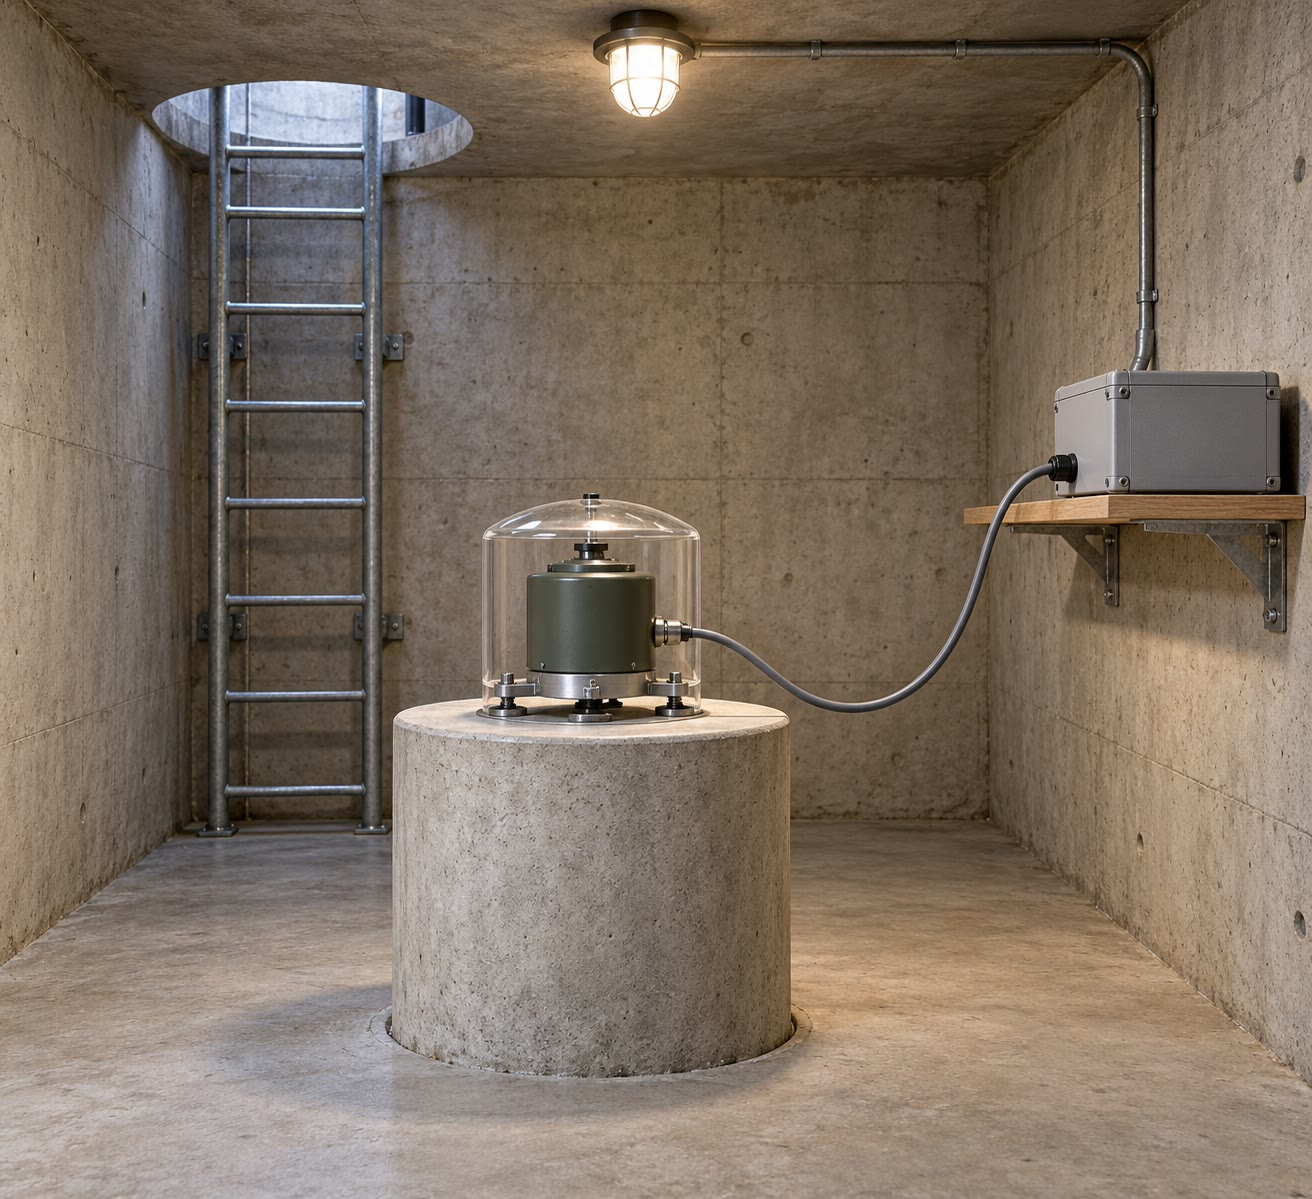
\includegraphics[width=\linewidth]{images/book3/ai/b1-seismometer-vault.jpg}

{\scriptsize भूमिगत कक्ष में अपने आधार पर एक ब्रॉडबैंड भूकंपमापी, दीवार पर लगे डेटा लॉगर के साथ (AI से बनाया गया चित्र)।}
\end{minipage}
\end{inthefield}

\section{अभ्यास}

\begin{exercise}[$\star$]\label{exo:b1:layered-earth:1}
PREM की त्रिज्याएँ $R = \qty{6371}{km}$, $r_{\text{CMB}} = \qty{3480}{km}$ और $r_{\text{ICB}} = \qty{1221.5}{km}$ लेकर, कोर और \omterm{def:b1:layered-earth:layers}{आंतरिक कोर} द्वारा घेरे गए पृथ्वी के आयतन के अंश परिकलित कीजिए।
% ledger: prem:cmb, prem:icb
\end{exercise}

\begin{exercise}[$\star$]\label{exo:b1:layered-earth:2}
\omterm{def:b1:layered-earth:discontinuity}{कोर–प्रावार सीमा} के ठीक ऊपर PREM $v_P = \qty{13.7166}{km.s^{-1}}$, $v_S = \qty{7.26466}{km.s^{-1}}$, $\rho = \qty{5.56645}{g.cm^{-3}}$ देता है; ठीक नीचे, $v_P = \qty{8.06482}{km.s^{-1}}$, $v_S = 0$, $\rho = \qty{9.90349}{g.cm^{-3}}$। सीमा के दोनों ओर सीमा-प्राचल और आयतन-मापांक (GPa में) परिकलित कीजिए। सीमा के आर-पार सबसे अधिक क्या बदलता है?
% ledger: data:prem, prem:cmb
\end{exercise}

\begin{exercise}[$\star$]\label{exo:b1:layered-earth:3}
\qty{30}{km} मोटी एक \omterm{def:b1:layered-earth:layers}{भूपर्पटी}, \qty{6.2}{km.s^{-1}} चाल से, \qty{8.1}{km.s^{-1}} वाले \omterm{def:b1:layered-earth:layers}{प्रावार} पर टिकी है। क्रांतिक कोण, क्रांतिक दूरी और \omterm{def:b1:layered-earth:head-wave}{क्रॉसओवर दूरी} परिकलित कीजिए।
\end{exercise}

\begin{exercise}[$\star$]\label{exo:b1:layered-earth:4}
कोर का द्रव्यमान \qty{1.94e24}{kg} और उसकी त्रिज्या \qty{3480}{km} है। \omterm{def:b1:layered-earth:discontinuity}{कोर–प्रावार सीमा} पर गुरुत्व परिकलित कीजिए और उसकी तुलना पृष्ठ-गुरुत्व \qty{9.82}{m.s^{-2}} से कीजिए। वह बड़ा क्यों है?
\end{exercise}

\begin{exercise}[$\star\star$]\label{exo:b1:layered-earth:5}
एक अपवर्तन-परिच्छेदिका पर पहले आगमन \qty{60}{km} पर \qty{10.0}{s} पर, \qty{200}{km} पर \qty{33.3}{s} पर और \qty{300}{km} पर \qty{45.8}{s} पर हैं; पहले बिंदु से गुज़रती रेखा मूल-बिंदु से होकर जाती है। $v_1$, $v_2$, अंतःखंड-समय और सीमा की गहराई ज्ञात कीजिए, और परिणाम को \omterm{def:b1:layered-earth:head-wave}{क्रॉसओवर दूरी} से जाँचिए।
\end{exercise}

\begin{exercise}[$\star\star$]\label{exo:b1:layered-earth:6}
दिखाइए कि एकसमान गोले का $I = 0.4\,MR^2$ है। फिर \qty{3480}{km} त्रिज्या और \qty{11.0}{g.cm^{-3}} घनत्व वाले एक कोर और \qty{4.45}{g.cm^{-3}} घनत्व वाले \omterm{def:b1:layered-earth:layers}{प्रावार} से बनी दो-परत पृथ्वी का द्रव्यमान और गुणांक $I/MR^2$ परिकलित कीजिए, जहाँ $R = \qty{6371}{km}$ है। उन्हें \num{5.972e24} kg और $0.3308$ से तुलना कीजिए।
\end{exercise}

\begin{exercise}[$\star\star$]\label{exo:b1:layered-earth:7}
\qty{1471}{km} गहराई पर PREM $v_P = \qty{12.16}{km.s^{-1}}$, $v_S = \qty{6.673}{km.s^{-1}}$, $\rho = \qty{4.86}{g.cm^{-3}}$ देता है, और गुरुत्व \qty{9.9}{m.s^{-2}} है। एडम्स–विलियम्सन समीकरण से दिया गया घनत्व-प्रवणता, \unit{g.cm^{-3}} में प्रति \qty{1000}{km}, परिकलित कीजिए, और उसकी तुलना PREM के घनत्वों से कीजिए: \qty{1471}{km} पर \num{4.844} और \qty{2471}{km} पर \num{5.357}।
% ledger: data:prem
\end{exercise}

\begin{exercise}[$\star\star$]\label{exo:b1:layered-earth:8}
\qty{670}{km} गहराई पर दाब का अनुमान लगाइए, जिसके लिए औसत घनत्व \qty{3.57}{g.cm^{-3}} और गुरुत्व \qty{9.9}{m.s^{-2}} है। वहाँ कौन-सा खनिज-परिवर्तन अपेक्षित है?
% ledger: frost:mantle-transitions
\end{exercise}

\begin{exercise}[$\star\star$]\label{exo:b1:layered-earth:9}
PREM के अनुसार \omterm{def:b1:layered-earth:layers}{बाह्य कोर} का औसत घनत्व \qty{10.90}{g.cm^{-3}} है; \omterm{def:b1:layered-earth:discontinuity}{आंतरिक-कोर सीमा} पर उसका घनत्व ऊपर \qty{12.166}{g.cm^{-3}} और नीचे \qty{12.764}{g.cm^{-3}} है। (क)~यदि उन्हीं परिस्थितियों में लोहा \omterm{def:b1:layered-earth:layers}{बाह्य कोर} से \qtyrange{5}{10}{\percent} अधिक घना है, तो वहाँ द्रव लोहे के लिए घनत्वों की कौन-सी परास बनती है? (ख)~\omterm{def:b1:layered-earth:discontinuity}{आंतरिक-कोर सीमा} पर घनत्व-छलांग प्रतिशत में परिकलित कीजिए, और उसकी तुलना हाल के अध्ययनों के \qty{4.5}{\percent} से कीजिए। (ग)~यदि छलांग अकेले जमने से बड़ी हो, तो वह हल्के तत्वों के बारे में क्या बताती है?
% ledger: badro:core, prem:icb
\end{exercise}

\begin{exercise}[$\star\star\star$]\label{exo:b1:layered-earth:10}
दिखाइए कि परावर्तित-तरंग समय $t_r(x) = \sqrt{x^2 + 4h^2}/v_1$ और \cref{thm:b1:layered-earth:two-layer} का हेड-तरंग समय $x = 2h\tan i_c$ पर बराबर हैं और उनकी ढलानें भी बराबर हैं, और उससे आगे $t_r > t_{\text{head}}$ है। व्याख्या कीजिए।
\end{exercise}

\begin{exercise}[$\star\star\star$]\label{exo:b1:layered-earth:11}
एकसमान घनत्व $\rho$ वाली एक पृथ्वी के लिए दिखाइए कि $g(r) = \tfrac43\pi G\rho r$ और $P(r) = \tfrac23\pi G\rho^2(R^2 - r^2)$ है। $\rho = \qty{5513}{kg.m^{-3}}$ और $R = \qty{6371}{km}$ लेकर केंद्रीय दाब परिकलित कीजिए, और उसकी तुलना PREM के \qty{363.85}{GPa} से कीजिए।
% ledger: earth:density, prem:centre
\end{exercise}

\begin{exercise}[$\star\star\star$]\label{exo:b1:layered-earth:12}
दिखाइए कि यदि परत में $g/\Phi$ स्थिर है, तो एडम्स–विलियम्सन समीकरण $\rho = \rho_0\exp\bigl(g(z - z_0)/\Phi\bigr)$ देता है, जहाँ $z$ गहराई है। इसे \omterm{def:b1:layered-earth:layers}{बाह्य कोर} पर लागू कीजिए, \qty{2891}{km} ($\rho_0 =
\qty{9.90}{g.cm^{-3}}$) से \qty{5149.5}{km} तक, औसत मानों $g = \qty{7.9}{m.s^{-2}}$ और $\Phi = \qty{87}{km^2.s^{-2}}$ के साथ; उसकी तुलना \omterm{def:b1:layered-earth:discontinuity}{आंतरिक-कोर सीमा} पर PREM के \qty{12.17}{g.cm^{-3}} से कीजिए।
% ledger: prem:icb
\end{exercise}

\section{समस्या: पृथ्वी के कोशों को तौलना}

\begin{problem}[{सप्ताहांत समस्या --- PREM से बनी चार-कोश पृथ्वी के आयतन, द्रव्यमान और जड़त्व-आघूर्ण; मापे गए द्रव्यमान और जड़त्व-आघूर्ण से तुलना; भीतर गुरुत्व और दाब}]
\label{pb:b1:layered-earth:1}
% values: calc/ch09.py; mean densities rounded from figdata prem_profiles (values part)
% ledger: data:prem, prem:constraints, prem:centre, prem:cmb, earth:mass, earth:MoI, const:G
पृथ्वी को PREM की त्रिज्याओं पर चार कोशों में काटा गया है, और हर एक को PREM का उसका औसत घनत्व, पूर्णांकित करके, दिया गया है:
\begin{center}
\small
\begin{tabular}{lccc}
\hline
कोश & से (km) & तक (km) & औसत घनत्व (\unit{g.cm^{-3}}) \\
\hline
\omterm{def:b1:layered-earth:layers}{भूपर्पटी}, ऊपरी \omterm{def:b1:layered-earth:layers}{प्रावार} और संक्रमण-क्षेत्र & 5701 & 6371 & 3.57 \\
निचला \omterm{def:b1:layered-earth:layers}{प्रावार} & 3480 & 5701 & 4.90 \\
\omterm{def:b1:layered-earth:layers}{बाह्य कोर} & 1221.5 & 3480 & 10.90 \\
\omterm{def:b1:layered-earth:layers}{आंतरिक कोर} & 0 & 1221.5 & 12.89 \\
\hline
\end{tabular}
\end{center}
$G = \qty{6.674e-11}{m^3.kg^{-1}.s^{-2}}$ लीजिए। पृथ्वी का मापा गया द्रव्यमान \qty{5.972e24}{kg} है और उसका जड़त्व-आघूर्ण-गुणांक $I/MR^2 = 0.3308$ है।

\medskip
\noindent\textbf{भाग I --- आयतन।}
\begin{enumerate}
  \item पृथ्वी का आयतन परिकलित कीजिए।
  \item प्रत्येक कोश का आयतन परिकलित कीजिए।
  \item प्रत्येक कोश कुल आयतन का कितना भाग घेरता है? कौन-सा कोश सबसे बड़ा है?
  \item कुल आयतन का कितना भाग कोर है?
\end{enumerate}

\noindent\textbf{भाग II --- द्रव्यमान।}
\begin{enumerate}[resume]
  \item प्रत्येक कोश का द्रव्यमान परिकलित कीजिए।
  \item उन्हें जोड़िए, और कुल की मापे गए द्रव्यमान से तुलना कीजिए।
  \item प्रतिरूप पृथ्वी का औसत घनत्व निकालिए।
  \item द्रव्यमान का कितना भाग \omterm{def:b1:layered-earth:layers}{आंतरिक कोर} में है?
  \item द्रव्यमान का कितना भाग \omterm{def:b1:layered-earth:layers}{प्रावार} और \omterm{def:b1:layered-earth:layers}{भूपर्पटी} में मिलाकर है?
  \item आयतन और द्रव्यमान में कोर के हिस्सों की तुलना कीजिए, और समझाइए।
\end{enumerate}

\noindent\textbf{भाग III --- जड़त्व-आघूर्ण।}
\begin{enumerate}[resume]
  \item \cref{prop:b1:layered-earth:integrals} से दिखाइए कि $r_1$ और $r_2$ के बीच एक समान कोश का $I = \tfrac{8\pi}{15}\rho\,(r_2^5 - r_1^5)$ है।
  \item प्रत्येक कोश का जड़त्व-आघूर्ण परिकलित कीजिए।
  \item कौन-सा कोश सबसे अधिक योगदान देता है, और \omterm{def:b1:layered-earth:layers}{आंतरिक कोर} लगभग कुछ क्यों नहीं जोड़ता?
  \item उन्हें जोड़िए और मॉडल के लिए $I/MR^2$ परिकलित कीजिए।
  \item $0.3308$ से और एक समान गोले के $0.4$ से तुलना कीजिए।
  \item हर वास्तविक कोश के भीतर घनत्व गहराई के साथ बढ़ता है। क्या यह समझाता है कि मॉडल का गुणांक बहुत अधिक क्यों है? समझाइए।
\end{enumerate}

\noindent\textbf{भाग IV --- गुरुत्व और दाब।}
\begin{enumerate}[resume]
  \item मॉडल की सतह पर गुरुत्व परिकलित कीजिए।
  \item \omterm{def:b1:layered-earth:discontinuity}{कोर–प्रावार सीमा} पर गुरुत्व परिकलित कीजिए।
  \item \omterm{def:b1:layered-earth:layers}{प्रावार} और \omterm{def:b1:layered-earth:layers}{भूपर्पटी} मिलाकर औसत घनत्व परिकलित कीजिए।
  \item \omterm{def:b1:layered-earth:layers}{प्रावार} में गुरुत्व \qty{10}{m.s^{-2}} के आसपास रहता है। \omterm{def:b1:layered-earth:discontinuity}{कोर–प्रावार सीमा} पर दाब का अनुमान लगाइए, और उसकी तुलना PREM के \qty{135.75}{GPa} से कीजिए।
  \item कोर का औसत घनत्व परिकलित कीजिए, और एक समान कोर में \omterm{def:b1:layered-earth:discontinuity}{कोर–प्रावार सीमा} से केंद्र तक दाब-वृद्धि, $\tfrac23\pi G\rho_c^2 r_c^2$ (\cref{exo:b1:layered-earth:11} को केवल कोर पर लागू करके) परिकलित कीजिए।
  \item दोनों को जोड़कर केंद्रीय दाब का अनुमान लगाइए, और PREM के \qty{363.85}{GPa} से तुलना कीजिए। अनुमान कम क्यों है?
  \item मॉडल की कौन-सी संख्याएँ किसी माप से जाँची जाती हैं, और कौन-सी केवल स्वयं PREM से?
  \item पृथ्वी के द्रव्यमान का कितना भाग कोर में है?
\end{enumerate}
\end{problem}
